\section{Menu}
\label{sec:imp_menu}

The menu is essential for navigating to specific options in the game. This section will cover how we calculate the (x,y) pixel and detect button clicks on the menu screens.

\subsection{Calculating Coordinates}

Before we can detect a button click, it is necessary that we modify the (x,y) coordinate provided when clicking on the canvas. To do this, we use the original (x,y) coordinate and subtract an offset, that is based on the size of the window the game is played in. This makes it possible to interact with the menu if the window in not full screen.

The offset for the $y$-coordinate is easy, since this does not change with the size of the window. It is always set to $50px$, which is subtracted from \verb|event.pageY| and put into the variable \verb|canvas_y|.\newline

The offset for the x-coordinate is a little more difficult. The calculation is shown below:

\begin{lstlisting}[language=JavaScript, caption=function: doMouseDown(event)]
	B = document.body;
	H = document.documentElement;
	width = Math.max( B.scrollWidth, B.offsetWidth, H.clientWidth, H.scrollWidth, H.offsetWidth);
	offset_x = Math.ceil((width-document.getElementById(this.gl.canvas).width)/2);
	offset_y = 50;
	canvas_x = event.pageX - offset_x;
	canvas_y = event.pageY - offset_y;
\end{lstlisting}
 
Line $3$ finds the max width of the window and stores it in \verb|width|. In line $4$ the offset is set to the width of the document subtracted by the width of the canvas (\verb|document.getElementById(this.gl.canvas).width|). The width of the canvas is retrieved dynamically, and since the canvas is centered, we divide by 2. We take the ceiling of the result to get a round number and \verb|canvas_x| is then set to the $x$-coordinate minus the offset in line $6$.

\subsection{Detecting Buttons}

Before discussion the detection of buttons, it should be noted, that in the final version of our game, the menu no longer have hexagon shaped buttons. This was done, because we did not like the initial look of the buttons, and it made the buttons click detection more difficult than needed. It would be more difficult, because of the hexagon shape instead of the implemented rounded square button, shown in \autoref{fig:final_menu}.

\begin{figure}[h]
	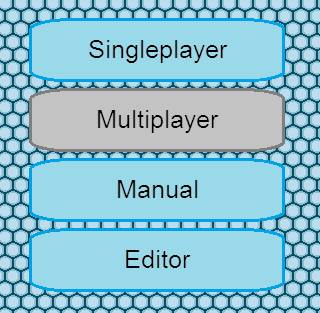
\includegraphics[width=\textwidth]{img/final_menu.png}
	\caption{Final design of the menu.}
	\label{fig:final_menu}
\end{figure}

Button clicks are defined as mouse events. To detect mouse events, a listener must be added to an element, which in this case is the canvas element, as seen below.

\begin{lstlisting}[language=JavaScript, caption=Add event listener to canvas]
canvas.addEventListener('mousedown', function(event)
	{
		game.doMouseDown(event);
	}, false);
\end{lstlisting}

In this case, when the \verb|mousedown| event is triggered, the function\\
\verb|doMousedown(event)| is called. \verb|doMouseDown()| first calculates the (x,y) coordinate with offsets as described in the previous subsection, and then calls the function \verb|checkButton(x, y)|, which is responsible for setting the new state of the game after a button is pressed. The state of the game is saved in the variable \verb|state|, which is a \verb|String|. There are two checks; one for the $x$-coordinate and one for the $y$. These checks depend on the size of the canvas and buttons. Below is shown the checks condition for the $x$-coordinate:

\begin{lstlisting}[language=JavaScript, caption=x condition check for menu buttons]
if(x <= this.gl.width/2-35+(this.spr_active_button.frame_width/2) && x >= this.gl.width/2-35-(this.spr_active_button.frame_width/2)){...}
\end{lstlisting}

\verb|this.gl.width| is the size of the canvas. To get the center, we divide by 2. Lastly we add and subtract half the width of the button, and $35px$, which is a variable that makes the button not appear in the complete center. A similar operation is done to the $y$-coordinate:

\begin{lstlisting}[language=JavaScript, caption=y condition check for menu buttons]
if(y >= this.gl.height/2-105-(this.spr_active_button.height/2) && y <= this.gl.height/2-105+(this.spr_active_button.frame_height/2)){...}
\end{lstlisting}

Here we focus on the height of the canvas and the height of the button. We add and subtract half the height of the button, which is $64px$ height. In this case, we are looking at the $y$ condition for button $1$, since we also subtract $105px$. The center of button $1$ is place $105px$ from the center of the canvas, button $2$ is placed $35px$ from the center of the canvas, button $3$ is placed $35px$ below the center, and button $4$ is place $105px$ below the center.\\

We have tried to make the calculation dynamic by using a minimum of absolute values to define the placement of the buttons and using the width and height of the canvas and buttons. We might have been able to calculate the $y$-placement of the buttons based on the height of the canvas and the amount of button we want a screen to include, so all buttons are evenly spaced between each other as in the current version. It is often a limitation to the program, if too many absolute values are used, since if one thing is changed, it might result in many changes throughout the program. A more dynamic program would not have this problem, if for example the width or height of the buttons changed or the number of buttons on a screen exceeds four, which is the maximum amount of buttons in the current version.

Just like the menu buttons, there also exist a back button and a home button, that work with similar boundary conditions, however we will not discuss this further. It should simply be noted, that the back button sets the state to the previous state and the home button sets the state as \verb|'Start'|, which is the home screen.